\section{Datentransformation}
\label{dt}
Die Daten -- in Form von Torschüssen -- wurden zuvor selektiert, bereinigt und anschließend auf eine relevante Zielmenge reduziert. In dieser Phase müssen diese Daten in eine adaptierte Form für die anschließende Regressionsanalyse transformiert werden, wozu einige der in \vref{dt} vorgestellten Methoden verwendet werden. Nachfolgend werden allgemeine Transformationen (vgl. \vref{at}), wie die des Koordinatensystems, sowie speziell für die Betrachtungswinkel (vgl. \vref{wdt} und \vref{kt}) ausgerichteten Transformationen durchgeführt, um ein passendes Format für die Verarbeitung in \gls{matlab} bereitstellen zu können.


\subsection{Allgemeine Transformationen}
\label{at}
Im Folgenden werden die allgemeinen Transformationen betrachtet, welche sowohl für die Betrachtung des Winkels und der Distanz zum Tor als auch in Bezug auf die Koordinaten des Schusses notwendig sind.

\paragraph{Unterscheidung zwischen Tor und Nicht-Tor} Nach der Datenreduzierung liegen die Datensätze wie im \vref{redData} abgebildeten Format vor, wobei die \textsf{type\_id} Aufschluss über das Resultat des Schusses gibt. Aus der \Vref{tab:events} lässt sich entnehmen, dass die Type-IDs \textsf{13, 14} und \textsf{15} einen Schuss ohne Torerfolg widerspiegeln, sowie die Type-ID \textsf{16} einen Torerfolg. Demzufolge wird das Attribut \textsf{type\_id} durch eine \textit{Codierung} in das Attribut \textsf{goal} transformiert, welches die numerischen Werte \textsf{0} für \textbf{Nicht-Tor} und \textsf{1} für \textbf{Tor} annimmt. \vref{atData} zeigt dazu exemplarisch das adaptierte Format der Schüsse aus \vref{redData}.

\paragraph{Transformation des Koordinatensystems}
Aus Anforderung 6 (vgl. \vref{tab:anf}) geht hervor, dass der Ursprungspunkt $P(0|0)$ der Funktion in der Mitte der gegnerischen Torauslinie liegen muss, sodass eine Transformation des Koordinatensystems nötig ist. Der Ursprungspunkt $P(0|0)$ liegt im  vorgegebenen Koordinatensystem von Opta (siehe \vref{opta_pitch}) in der eigenen Spielhälfte (links) auf dem unteren Eckstoßpunkt und muss, wie in \vref{transf_pitch} dargestellt, verschoben werden. Zusätzlich werden die Achsen umgekehrt, wodurch sich folgende Transformationsregeln der x- und y-Koordinate ergibt:\enlargethispage{\baselineskip}\newline

\centerline{$\boldsymbol{x_{neu}} \Rightarrow$ y - 50 }
\centerline{$\boldsymbol{y_{neu}} \Rightarrow$ |x - 100|}

Diese Transformationsregeln werden so angewendet, dass die jeweiligen x- und y-Werte in numerischer Form aktualisiert vorliegen. Da beide Koordinatenwerte gleich skaliert sind, ist keine \textit{Normalisierung} der Attribute notwendig.

\begin{figure}[H]
\centering
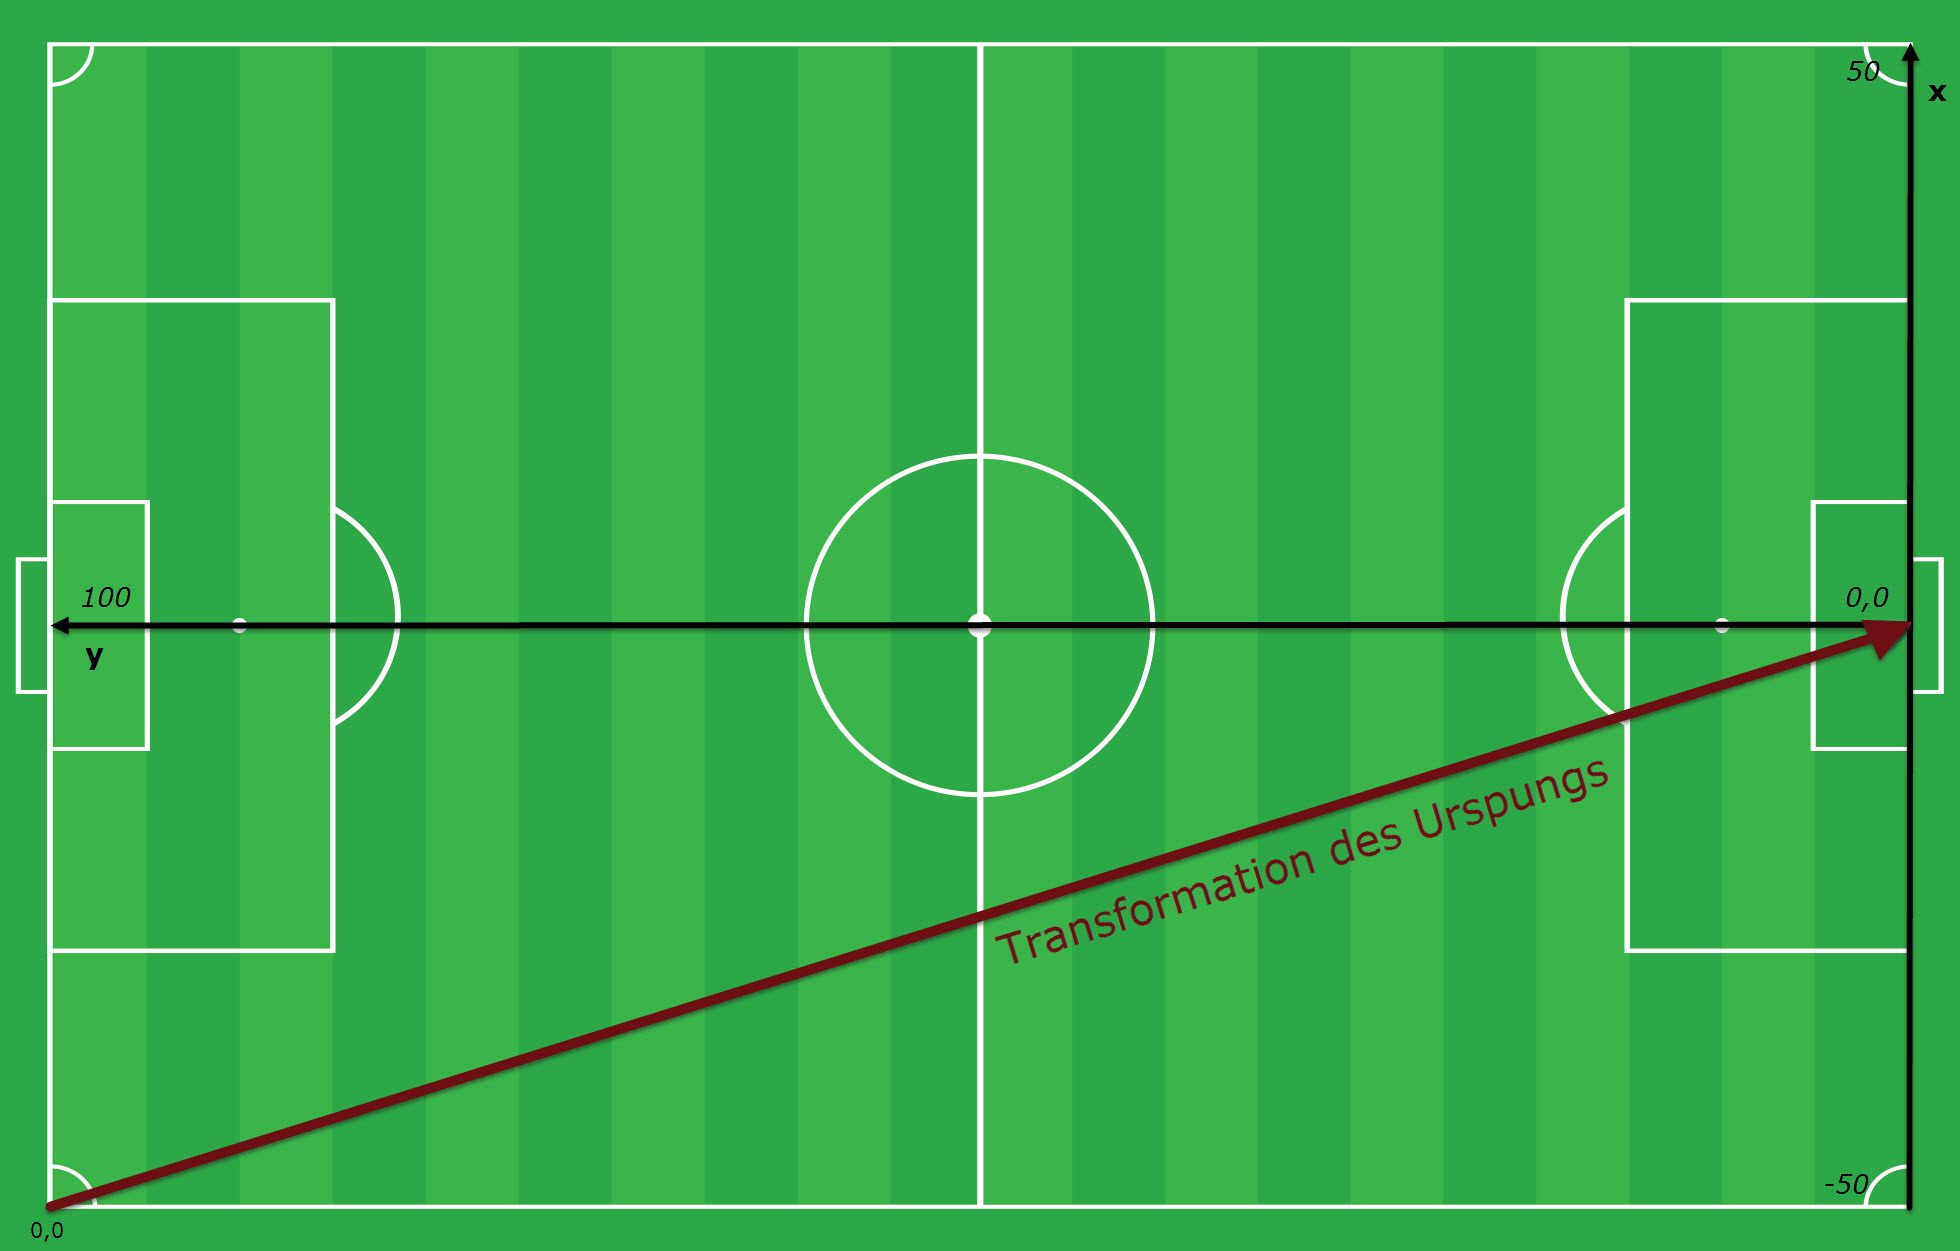
\includegraphics[scale=0.27]{se-wa-jpg/transf_pitch}
\caption[Transformation des Koordinatensystems]{Transformation des Koordinatensystems}
\label{transf_pitch}
\end{figure}

\enlargethispage{2\baselineskip} Folglich ergibt sich nach diesen Transformationen eine neue Struktur der Datensätze, die in Bezug auf die Daten aus \vref{redData} im \vref{atData} dargestellt sind.\newline

\captionListing{Struktur der Daten nach der allgemeinen Transformation}
\begin{lstlisting}[caption=\captionListingText,language=json,xleftmargin=5mm,label=atData] 
[
	{
		"goal": 1,
		"x": -6.5,
		"y": 5
	},
	{
		"goal": 0,
		"x": 25.9,
		"y": 10.8,
	},
	...
]
\end{lstlisting}

\subsection{Transformation für Koordinatenbetrachtung}
\label{kt}
Um die Laufzeit der Regressionsanalyse (vgl. \vref{bk}) innerhalb von MATLAB zu reduzieren, gilt es die Datenmenge zu komprimieren. Die Datenaggregation ist hierbei jedoch auch aus inhaltlichen Gründen sinnvoll, da die Schüsse auf einer zu detaillierten Ebene vorliegen (jeder Schussversuch wird einzeln betrachtet). Hierzu wird das Spielfeld zunächst in Raster der Größe \textsf{1x1} (Maßstab der Koordinatenwerte) eingeteilt, wie in \vref{raster} verdeutlicht. Diese Einteilung bietet die Möglichkeit eine komprimierte und gleich gewichtete Aussagekraft über die Wahrscheinlichkeit eines Torerfolges innerhalb jedes Rasters zu treffen.

\begin{figure}[H]
\centering
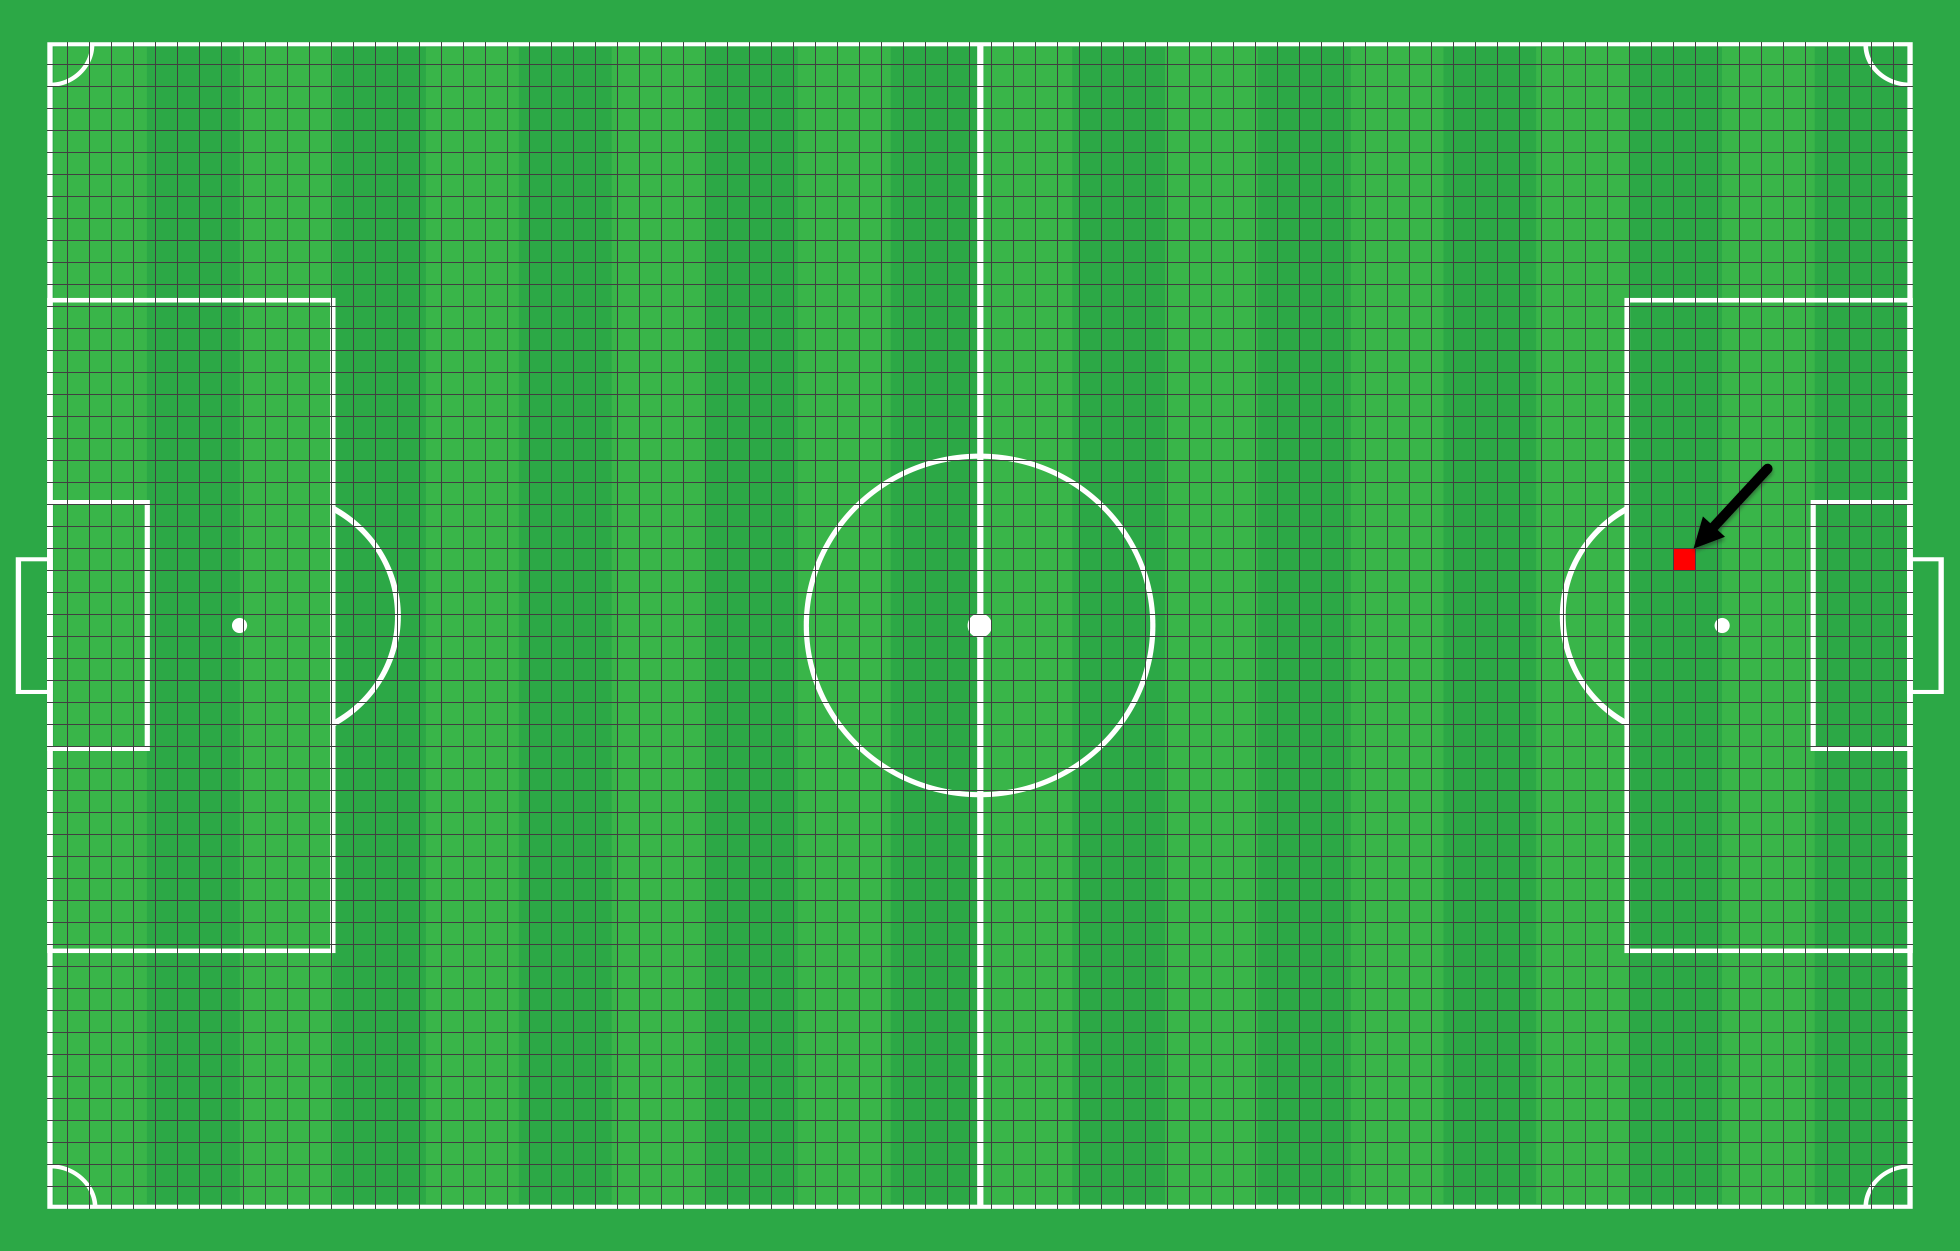
\includegraphics[scale=0.28]{se-wa-jpg/raster}
\caption[Einteilung des Spielfeldes in Raster]{Einteilung des Spielfeldes in Raster}
\label{raster}
\end{figure}

Betrachtet man dazu alle Schussversuche die im rot markierten Raster liegen, so kann durch die \vref{rh}, mit Hilfe der relativen Häufigkeit, die Wahrscheinlichkeit $p$ ermittelt werden. Sollten keine Schüsse innerhalb eines Rasters vorliegen, wird automatisch die Wahrscheinlichkeit 0 angenommen.

\begin{equation}
p = \frac{Anzahl~der~Tore~im~Raster}{Gesamtzahl~der~Schussversuche~im~Raster}
\label{rh}
\end{equation}

Nachdem alle Schussversuche eingeteilt und die einzelnen relativen Häufigkeiten der Raster berechnet wurden, kann aus der \vref{tab:dak} die Wahrscheinlichkeit für jede beliebige Kombination aus x- und y-Koordinate ($p_{xy})$ abgelesen werden.\footnote{Die Koordinatenwerte werden jeweils aufgerundet.} Dabei gilt für die x-Koordinate der Wertebereich $-50 \le m \le 50$ und für die y-Koordinate $1 \le k \le 100$. Für die Spiegelung (vgl. Anforderung 7 in \vref{tab:anf}) des Spielfeldes entlang der y-Achse wird die durchschnittliche Wahrscheinlichkeit aus den gegenüberliegenden Raster ($Q(x,y)$) herangezogen. Beispielsweise wird hierzu die Wahrscheinlichkeit \textsf{1} aus $Q(-5,10)$ mit der Wahrscheinlichkeit \textsf{0} aus $\overline{Q}(5,10)$ summiert und anschließend durch zwei geteilt, um den Mittelwert \textsf{0.5} zu erhalten. 


%%%%%%%%%%%%%%%%%% Aggregation Koordinaten %%%%%%%%%%%%%%%%%%
\tablefirsthead{\hline\multicolumn{6}{|c|}{\textbf{Datenaggregation Koordinaten}}\\\hline\hline Koordinaten & \textsf{$x_1$} & \textsf{$x_2$} & \textsf{$x_3$} & \textsf{...} & \textsf{$x_m$}\\\hline}
\tablehead{\hline Koordinaten & \textsf{$x_1$} & \textsf{$x_2$} & \textsf{$x_3$} & \textsf{...} & \textsf{$x_m$}\\}
\tabletail{\hline \multicolumn{3}{|r|}{\textsl{Fortsetzung nächste Seite}}\\\hline }
\tablelasttail{}
\bottomcaption{Datenaggregation für die Koordiantenbetrachtung\label{tab:dak}}
\begin{center}%
\begin{supertabular}{ | P{3.2cm} | P{1.5cm} | P{1.5cm} | P{1.5cm} | P{1.5cm} |  P{1.5cm} |}
\textsf{$y_1$}	&   $p_{11}$	& 	$p_{12}$  &  $p_{13}$  &  ... &  $p_{1m}$\\
\hline
\textsf{$y_2$}	&   $p_{21}$	& 	$p_{22}$  &  $p_{23}$  &  ... &  $p_{2m}$\\
\hline
\textsf{$y_3$}	&   $p_{31}$	& 	$p_{32}$  &  $p_{33}$  &  ... &  $p_{3m}$\\
\hline
\textsf{...}	&   ...	        & 	...       &  ...        &  ... & ...\\
\hline
\textsf{$y_k$}	&   $p_{k1}$	& 	$p_{k2}$  &  $p_{k3}$  &  ... &  $p_{km	}$\\
\hline
\end{supertabular}
\end{center}




\subsection{Transformation für Winkel- und Distanzbetrachtung}
\label{wdt}
Für die Betrachtung der Wahrscheinlichkeit in Abhängigkeit des Winkels und der Distanz des Schusses\footnote{Es wird der Punkt vom dem der Schuss ausgeht genommen.} zum Tor, müssen zunächst die Koordinaten durch mathematische Berechnungen transformiert werden. Die Distanz kann dabei mit Hilfe des \textit{Satz des Pythagoras} -- in umgestellter Form der \vref{distanz} -- ermittelt werden. Die x- und y-Koordinaten, sowie die Distanz bilden das in \vref{winkel_distanz} dargestellte rechtwinkligen Dreiecks. 

\begin{equation}
\label{distanz}
Distanz= \sqrt{x^2 + y^2}
\end{equation}

Zur Berechnung des Winkels wird zunächst festgelegt, dass ein Schuss aus zentraler Position zum Tor den Winkel $0^\circ$ und ein Schuss von der Torauslinie einen Winkel von $90^\circ$ widerspiegelt. \vref{winkel_distanz} verdeutlicht diese Annahme, wobei es keine \glqq negativen\grqq~Winkel gibt, sodass immer der Betrag der x-Koordinate herangezogen wird. Somit werden beide Seiten des Spielfeldes automatisch gespiegelt und Anforderung 7 (vgl. \vref{tab:anf}) erfüllt. Durch die Anwendung des \textit{Arkustangens} in \vref{winkel} kann innerhalb des rechtwinkligen Dreiecks der Winkel von der Position des Schusses zum Tor berechnet werden.

\begin{equation}
\label{winkel}
Winkel= \arctan(\frac{|x|}{y})
\end{equation}

Die \vref{winkel_distanz} verdeutlicht diese Berechnungen nochmals anhand einer Skizze mit der eingezeichneten Distanz und Winkel des Schussversuches (rotes Kreuz).

\begin{figure}[H]
\centering
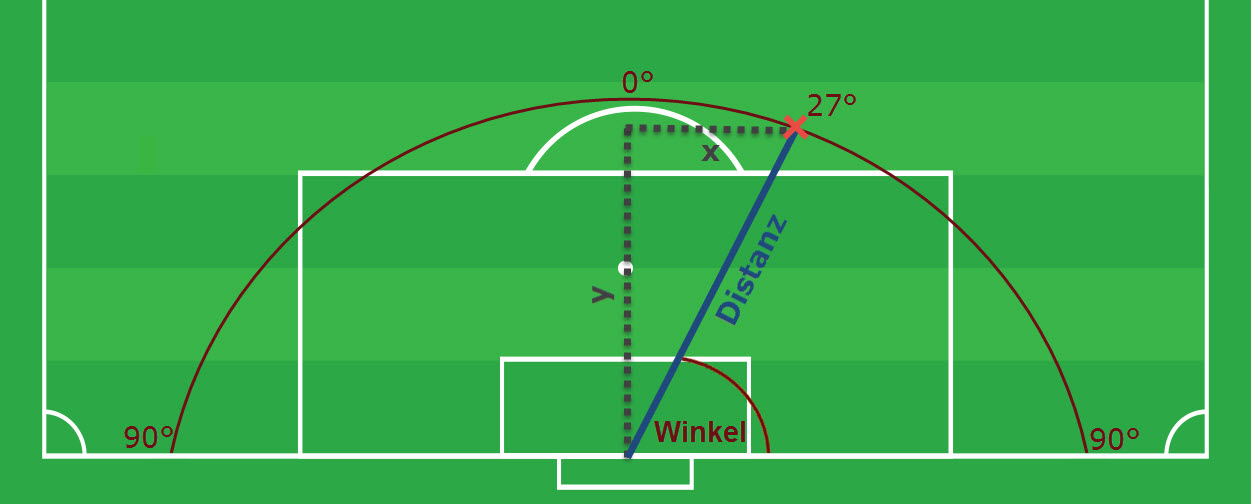
\includegraphics[scale=0.45]{se-wa-jpg/winkel_distanz}
\caption[Berechnung der Distanz und des Winkels]{Berechnung der Distanz und des Winkels}
\label{winkel_distanz}
\end{figure}

Das \vref{wdData} zeigt hierzu die resultierende Struktur der Daten nach der Transformation der Koordinaten in die Winkel- und Distanzwerte anhand der Schüsse aus \vref{atData}.\newline

\captionListing{Struktur der Daten für die Winkel- und Distanzbetrachtung}
\begin{lstlisting}[caption=\captionListingText,language=json,xleftmargin=5mm,label=wdData] 
[
	{
		"goal": 1,
		"angle": 52.4,
		"distance": 8.2
	},
	{
		"goal": 0,
		"angle": 67.4,
		"distance": 28.1,
	},
	...
]
\end{lstlisting}

Wie bei der zuvor dargestellten Rastereinteilung der Koordinaten, werden auch hier die Attribute \textit{Distanz} (mit $1 \le m \le 100$) und \textit{Winkel} (mit $0 \le k \le 90$) in Intervalle der Größe 1 eingeteilt und die Schussversuche in diese Gruppen eingeordnet. Winkel- und Distanzwert werden wie die Koordinaten zuvor dabei immer aufgerundet. Anschließend wird für jede Gruppierung mit Hilfe der relativen Häufigkeit die Wahrscheinlichkeit $p$ ermittelt, in dem die Anzahl der Schüsse mit resultierendem Torerfolg durch die Gesamtzahl der Schussversuche geteilt wird (vgl. \vref{rh}). Folglich kann für jede Kombination der Attributwerte aus Distanz und Winkel eine Wahrscheinlichkeit ($p_{wd}$) bestimmt werden, die aus \vref{tab:dawd} abgelesen werden kann. Die Schüsse aus \vref{wdData} würden dementsprechend in die Kombinationen $p_{53,9}$ bzw. $p_{68,29}$ eingruppiert werden.


%%%%%%%%%%%%%%%%%% Aggregation Winkel und Distanz %%%%%%%%%%%%%%%%%%
\tablefirsthead{\hline\multicolumn{6}{|c|}{\textbf{Datenaggregation Winkel und Distanz}}\\\hline\hline Winkel/Distanz & \textsf{$d_1$} & \textsf{$d_2$} & \textsf{$d_3$} & \textsf{...} & \textsf{$d_m$}\\\hline}
\tablehead{\hline Winkel/Distanz & \textsf{$d_1$} & \textsf{$d_2$} & \textsf{$d_3$} & \textsf{...} & \textsf{$d_m$}\\}
\tabletail{\hline \multicolumn{6}{|r|}{\textsl{Fortsetzung nächste Seite}}\\\hline }
\tablelasttail{}
\bottomcaption{Datenaggregation für die Winkel- und Distanzbetrachtung\label{tab:dawd}}
\begin{center}%
\begin{supertabular}{ | P{3.2cm} | P{1.5cm} | P{1.5cm} | P{1.5cm} | P{1.5cm} |  P{1.5cm} |}
\textsf{$w_1$}	&   $p_{11}$	& 	$p_{12}$  &  $p_{13}$  &  ... &  $p_{1m}$\\
\hline
\textsf{$w_2$}	&   $p_{21}$	& 	$p_{22}$  &  $p_{23}$  &  ... &  $p_{2m}$\\
\hline
\textsf{$w_3$}	&   $p_{31}$	& 	$p_{32}$  &  $p_{33}$  &  ... &  $p_{3m}$\\
\hline
\textsf{...}	&   ...	        & 	...       &  ...        &  ... & ...\\
\hline
\textsf{$w_k$}	&   $p_{k1}$	& 	$p_{k2}$  &  $p_{k3}$  &  ... &  $p_{km	}$\\
\hline
\end{supertabular}
\end{center}





